\documentclass[fyp]{socreport}

% %\usepackage{ctex}
%\usepackage[center]{titlesec}%章节标题位置
% \usepackage[BoldFont,SlantFont,CJKchecksingle]{xeCJK}

\usepackage{threeparttable}
\usepackage{booktabs}
\usepackage{graphicx}

\usepackage{amsmath}
\usepackage{amsfonts}
\usepackage{bm}%bold form in math environment
 %\sideset{}{}\sum  求和符号左上角,右上角添加标记
\usepackage{graphicx}
\usepackage{wrapfig}
\usepackage{subfigure}%多图共用caption
%\usepackage[version=3]{mhchem} %化学式  \ce{*} 见数字均为下标
% \usepackage[CJKbookmarks,bookmarksnumbered,
%                      bookmarksopen,colorlinks,citecolor=blue,
%                      linkcolor=blue]{hyperref}%链接样式
\usepackage{geometry}
\usepackage{fontspec,xunicode,xltxtra}
\usepackage{titlesec}
\usepackage{indentfirst}
\usepackage{multicol}
\usepackage{amssymb}
\usepackage{amsthm}
%\usepackage{mathabx}
\usepackage{multirow}
\usepackage{diagbox}
%\usepackage{fixltx2e}%解决caption中使用向量的问题配合命令\MakeRobust{\overrightarrow}
%\usepackage{exercise}
\usepackage{fancyhdr}
\usepackage{titling}%调整title
\usepackage{tabu,tikz}
\usepackage{setspace} 
\usepackage{pdfpages} %insert pdf
\usepackage{textcomp} %support other codes
\usepackage{listings} %codes support
\usepackage{xcolor}
\usepackage{url}
%\usepackage{blindtext}%?
%\usepackage[svgnames]{xcolor} % Required to specify font color

% \XeTeXlinebreaklocale "zh"
%\XeTeXlinebreakskip = 0pt plus 1pt minus 0.1pt
\geometry{top=25mm,bottom=20mm,left=30mm,right=30mm}%调整正文上下边距
\chead{\zhongsong 华中科技大学本科生毕业设计(论文)开题报告}                                                                                                
\renewcommand{\headrulewidth}{1pt}  %页眉线宽,设为0可以去页眉线
\lhead{}%页眉左边
\rhead{}%页眉右边
%\oddsidemargin=11mm
%\evensidemargin=5mm
\setCJKmainfont{SimSun}
\setCJKmonofont{SimSun}
\setmainfont{Times New Roman}
\fontsize{10.5pt}{15.7pt}\selectfont
\graphicspath{{Titlepage/}{Sect1/}{Sect2/}{Sect3/}{Sect4/}}
%\numberwithin{equation}{section}

\pagestyle{fancy}
%-------调整表格线条粗细-------
%\newcolumntype{L}[1]{>{\vspace{0.5em}\begin{minipage}{#1}\raggedright\let\newline\\
%\arraybackslash\hspace{0pt}}m{#1}<{\end{minipage}\vspace{0.5em}}}
%\newcolumntype{R}[1]{>{\vspace{0.5em}\begin{minipage}{#1}\raggedleft\let\newline\\
%\arraybackslash\hspace{0pt}}m{#1}<{\end{minipage}\vspace{0.5em}}}
%\newcolumntype{C}[1]{>{\vspace{0.5em}\begin{minipage}{#1}\centering\let\newline\\
%\arraybackslash\hspace{0pt}}m{#1}<{\end{minipage}\vspace{0.5em}}}
%\makeatletter
%\def\hlinewd#1{%
%  \noalign{\ifnum0=`}\fi\hrule \@height #1 \futurelet
%   \reserved@a\@xhline}
%\makeatother
%--------------------------------

% \def\degree{${}^{\circ}$}
% \def\ee{\mathrm{e}}%自然对数底数
% \def\ii{\mathrm{i}}%复数单位
% \def\dd{\mathrm{d}}
% \def\pp{\partial}
% \def\z{\left}
% \def\y{\right}
% \def\ol{\overline}
% \def\ora{$\overrightarrow{}$}

%----------字体相关----------
\setCJKfamilyfont{song}{SimSun}
\newcommand{\song}{\CJKfamily{song}} 
\setCJKfamilyfont{hei}{SimHei}
\newcommand{\heiti}{\CJKfamily{hei}}
\setCJKfamilyfont{zs}{STZhongsong}
\newcommand{\zhongsong}{\CJKfamily{zs}}
\setCJKfamilyfont{kai}{KaiTi}
\newcommand{\kaishu}{\CJKfamily{kai}} 
\newfontfamily\Rom{Times New Roman}
\setlength{\baselineskip}{0em}
\newcommand{\chuhao}{\fontsize{42pt}{\baselineskip}\selectfont}     %初号  
\newcommand{\xiaochuhao}{\fontsize{36pt}{\baselineskip}\selectfont} %小初号  
\newcommand{\yihao}{\fontsize{28pt}{\baselineskip}\selectfont}      %一号  
\newcommand{\erhao}{\fontsize{21pt}{\baselineskip}\selectfont}      %二号  
\newcommand{\xiaoerhao}{\fontsize{18pt}{\baselineskip}\selectfont}  %小二号  
\newcommand{\sanhao}{\fontsize{15.75pt}{\baselineskip}\selectfont}  %三号  
\newcommand{\sihao}{\fontsize{14pt}{18pt}\selectfont}%     四号  
\newcommand{\xiaosihao}{\fontsize{12pt}{18pt}\selectfont}  %小四号  
\newcommand{\wuhao}{\fontsize{10.5pt}{15.7pt}\selectfont}    %五号  
\newcommand{\xiaowuhao}{\fontsize{9pt}{13pt}\selectfont}   %小五号  
\newcommand{\liuhao}{\fontsize{7.875pt}{\baselineskip}\selectfont}  %六号  
\newcommand{\qihao}{\fontsize{5.25pt}{\baselineskip}\selectfont}    %七
%\newcommand{\bb}[1]{\raisebox{-2ex}[0pt][0pt]{\shortstack{#1}}}% 表格中向下移动文字2ex
\renewcommand{\abstractname}{\xiaoerhao \heiti \textbf{摘~~要}}
\renewcommand{\contentsname}{\xiaoerhao \heiti \textbf{目~~录}}
\renewcommand{\figurename}{\wuhao\kaishu 图}
\renewcommand{\tablename}{\wuhao\kaishu 表}
\renewcommand\refname{\sihao \song \textbf{参考文献}}
%\renewcommand{\thesubsection}{\Alph{subsection}}
\titleformat{\section}{\sihao \song \bf}{\thesection}{1em}{}
\titleformat{\subsection}{\xiaosihao \song \bf}{\thesubsection}{1em}{}
%\MakeRobust{\overrightarrow}%解决caption中使用向量的问题配合命令\usepackage{fixltx2e}
%\MakeRobust{\vv}
%
%\makeatletter
\def\fnum@figure#1{\figurename\nobreakspace\thefigure\hspace{1em}}% 去掉图后面的冒号并加空白空1em
\def\fnum@table#1{\tablename\nobreakspace\thetable\hspace{1em}}% 去掉表后面的冒号并加空白1em
%\makeatother

\hypersetup{colorlinks=false,pdfborder=0 0 0} 
%\setcounter{tocdepth}{2}

%\setlength{\droptitle}{-4em}     % Eliminate the default vertical space
%\addtolength{\droptitle}{-20mm}



\usepackage{threeparttable}
\usepackage{booktabs}
\usepackage{graphicx}
\usepackage{multirow}
\usepackage{titlesec}
\usepackage{enumitem}

\usepackage[colorlinks,linkcolor=black]{hyperref}


\usepackage{fullpage}
\begin{document}
\pagenumbering{roman}
\title{A BERT-Based Framework for Targeted Sentiment Analysis}
\author{Xiang Pan}
\projyear{2020/04}
\projnumber{CP3106}


\advisor{Prof. Lee Wee Sun}
\deliverables{
	\item Report: 1 Volume
	\item Source Code: 1 DVD}
\maketitle
\begin{abstract}
Sentiment Analysis 
In the report, we distinguish the differences between the general sentiment analysis and Targeted Sentiment Analysis. Future more, we analyze the existing problems of Targeted Sentiment Analysis. To address these problems, we proposed a new BERT-based framework to solve the targeted sentiment analysis problem. Based on the framework, we introduce some auxiliary training methods to improve the accuracy of the results. To illustrate the existing methods' robustness problem toward new unseen targets, we introduce a new data set setting, which explicitly make the targets in the training set and test set to be different. Then, we use the adversarial training methods to enhance the robustness of our framework training. Overall, our framework behave better than the state of the art in the traditional targeted sentiment analysis setting and showed robustness in the new re-split data set setting.Finally, we describe the future work in targeted sentiment analysis.


\begin{descriptors}
    \item C5 Computer System Implementation
	\item G2.2 Graph Algorithms
\end{descriptors}
\begin{keywords}
	Targeted Sentiment Analysis, robustness, BERT, adversarial training, auxiliary training
\end{keywords}
\begin{implement}
	Python, Pytorch, RTX 2080TI
\end{implement}
\end{abstract}

\begin{acknowledgement}
   I would like to thank my friends, families, members of the laboratory and advisors.
   Without them, I would not have be able to complete this project.
%    In addtion, thanks to the NGNE program for giving me a opportunity to do research.
\end{acknowledgement}

\listoffigures 
\listoftables
\tableofcontents 

\chapter{Introduction}
The sentiment analysis is a specific task under the text classification.




Many problems exist in computer science.  In this project, we 
studied one particular important problem and propose a solution 
for it.  

\section{Background}
In this section, we briefly discuss the history and background
of the targeted sentiment analysis problem.  A detail literature survey is presented in 
Chapter \ref{ch:related}.

The sentiment analysis was proposed
The problem we study in this report is an important one.
This problem is first proposed in 1990 in the context
of graph theory \cite{smith90graph}.  Zhang gives thec
first algorithm to the problem and applied it to solve several 
problems in artificial intelligence \cite{zhang91ai,zhang92ai}.  
More recently, a slightly different formulation of the problem
is studied independently \cite{kovsky92diff,ali94diff}.  None of this previous work
uses the technique that we propose in this project.  Thus, we 
believe that our algorithm is novel.

\section{The Problem}
In this section, we formally defined the problem.  We adopt
the definition given by Kovsky \cite{kovsky92diff}.

\section{Our Solution}
\section{Report Organization}

\chapter{Related Work}
\label{ch:related}


\section{Text classification}



\section{Aspect Based Sentiment Analysis}

\section{Pre-trained models}







\chapter{Problem and Algorithm}
\section{Formal Description of Problem}
Given a text sequence with n words text=$\{w_1,w_2,w_3,w_4,...,w_n\}$ and a target with m words, target text=  $\{t_1,t_2,t_m\}$ with its begin position $b$, the problem is to classify the sentiment polarity $polarity=\{positive,neutral,negative\}$ towards the given target in the context. We followed the SemEval 2014 Task 4\cite{pontiki-etal-2014-semeval}




\section{Design of Algorithm}
\section{A general framework for Targeted Sentiment Analysis(TSA)}

\subsection{BERT for text classification}


As a powerful pre-trained universal language model, BERT can be used in various downstream tasks.
To utilize bert, we have several direct ways:
\begin{enumerate}
    \item Using BERT embeddings as the input of sequence
    \item Fine-tuned BERT by [CLS] classification token.
\end{enumerate}

To enhance the performance, \cite{sun2019finetune} have several methods for text classification: 


\paragraph{Trick for text classification}

\begin{enumerate}
    \item Various fine tuning methods
    \begin{enumerate}
        \item Within-task pre-training
        \item In-domain pre-training
        \item Cross-domain pre-training
    \end{enumerate}
    
    \item Different learning rates are used for different layers of Bert
\end{enumerate}


Those methods only consider the sentence-level classification. For TSA, the classification problem is more fine-grained, hence we will introduce our BERT-based framework for TSA.


\subsubsection{BERT for TSA}

As described in the related work, BERT-SPC \cite{Song2019} repeat the target words at the end of context sentence. 

\begin{figure}[h]
    \centering
    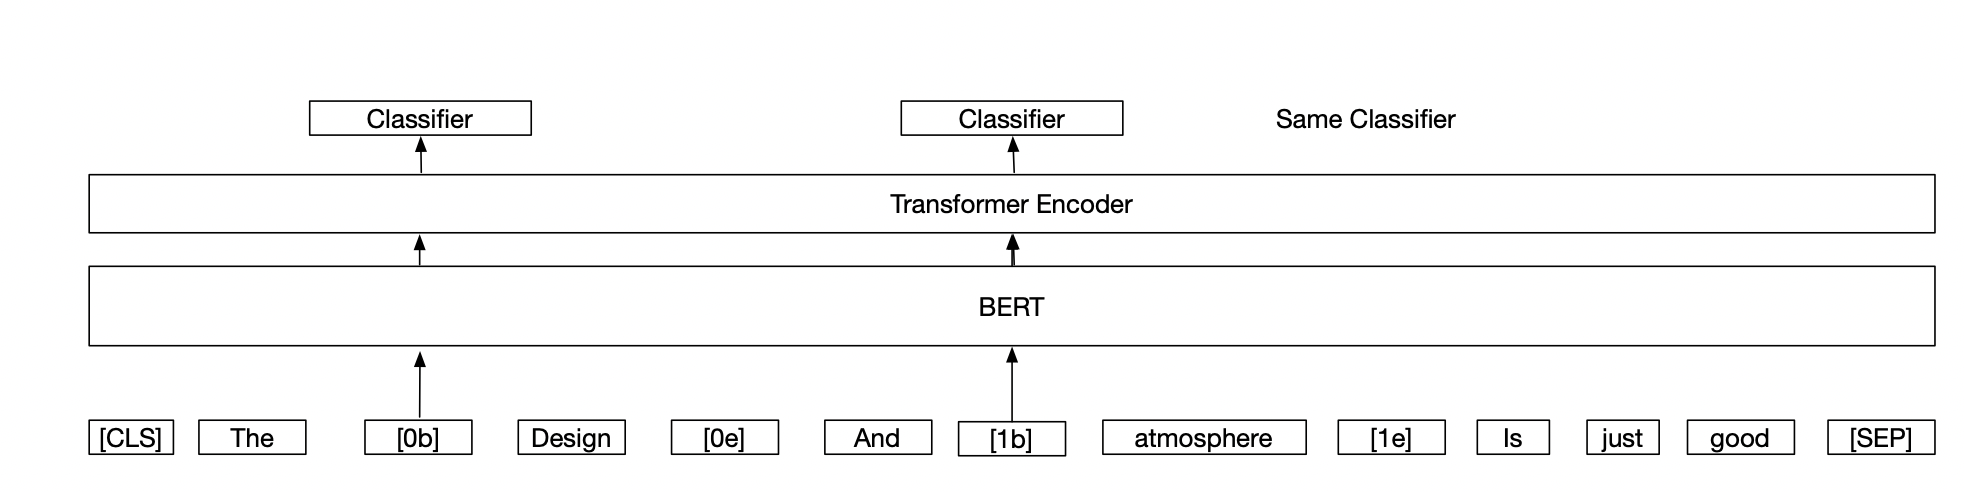
\includegraphics[width=\linewidth]{./image/Framework.png}
    \caption{Our framework for TSA}
  \label{Framework}
\end{figure}

For original bert, the most direct way to utilize bert

As show in the image \ref{Framework}, we add the begin token and end token around the target. In our initial experiments, we add the same token for different targets in the context sentence. However, 





\section{Auxiliary training methods for TSA}


\section{Adversarial training methods for Robustness of TSA}




% \section{Proof of Correctness}
% \section{Complexity Analysis}

\chapter{Evaluation}


\section{Implementation Details}
Our experiment is based on the code of \href{https://github.com/songyouwei/ABSA-PyTorch}{ABSA-Pytorch}. 
We release our code in \href{https://github.com/Xiang-Pan/ABSA-PyTorch}{TSA-Pytorch}.
\section{Experimental Setup}

\subsection{Targeted Sentiment Analysis}

\subsection{Domain Adaption' effect on Targeted Sentiment Analysis}


\subsection{Robustness of Targeted Sentiment Analysis Algorithms}











\section{Visualization}
\subsection{Pre-trained BERT Visualization}


\subsection{Fine-tuned BERT Visualization}


\subsection{Conclusion from Visualization}




\section{Results}


\begin{table*}[tp]
    \small
    \centering
    \resizebox{\textwidth}{!}{
    \begin{threeparttable}
    \caption{
		Test results on three typical data sets.
		% The baselines results are from the existed paper's reports. \\
		% '-' means do not include included in the original paper or the test can not be done in this data set. 
		% The highest score is marked with \textbf{bold}.
	}
      \begin{tabular}{cccccccc}
      \toprule
      \multirow{2}{*}{ }&\multirow{2}{*}{\textbf{Models}}&
      \multicolumn{2}{c}{\textbf{Twitter}}&\multicolumn{2}{c}{\textbf{Restaurant}}&\multicolumn{2}{c}{\textbf{Laptop}}\cr
      \cmidrule(lr){3-4} \cmidrule(lr){5-6} \cmidrule(lr){7-8}
      &&Accuracy&Macro-F1&Accuracy&Macro-F1&Accuracy&Macro-F1\cr
      \midrule
          \multirow{4}*{\textbf{RNN baselines}}
          &TD-LSTM           &0.7080&0.6900              &0.7563&-                  &0.6813&-         \cr
          &ATAE-LSTM         &-&-                        &0.7720&-                  &0.6870&-         \cr
          &IAN               &-&-                        &0.7860&-                  &0.7210&-         \cr
          &RAM               &0.6936&0.6730              &0.8023&0.7080             &\textbf{0.7449}&\textbf{0.7135}     \cr
      \midrule
          \multirow{3}*{\textbf{Non-RNN baselines}}
          &Feature-based SVM &0.6340&0.6330              &0.8016&-                  &0.7049&-           \cr
          &Rec-NN            &0.6630&0.6590              &-&-                       &-&-              \cr
          &MemNet            &0.6850&0.6691              &0.7816&0.6583             &0.7033&0.6409    \cr
      \midrule
          \multirow{4}*{\textbf{AEN-GloVe ablations}}
          &AEN-GloVe w/o PCT       &0.7066&0.6907              &0.8017&0.7050             &0.7272&0.6750 \cr
          &AEN-GloVe w/o MHA       &0.7124&0.6953              &0.7919&0.7028             &0.7178&0.6650 \cr
          &AEN-GloVe w/o LSR       &0.7080&0.6920              &0.8000&0.7108             &0.7288&0.6869 \cr
          &AEN-GloVe-BiLSTM        &0.7210&\textbf{0.7042}     &0.7973&0.7037             &0.7312&0.6980 \cr
      \midrule
          \multirow{3}*{\textbf{Ours}}
          &AEN-GloVe  &\textbf{0.7283}&0.6981  &\textbf{0.8098}&\textbf{0.7214}  &0.7351&0.6904 \cr
          &BERT-SPC  &\textbf{0.7355}&\textbf{0.7214} &\textbf{0.8446}&\textbf{0.7698} &\textbf{0.7899}&\textbf{0.7503} \cr
          &AEN-BERT &\textbf{0.7471}&\textbf{0.7313} &\textbf{0.8312}&\textbf{0.7376} &\textbf{0.7993}&\textbf{0.7631} \cr
      \bottomrule
      \end{tabular}fr
      \label{tab:result}
      \end{threeparttable}}
  \end{table*}

%  asdfsdaf \cite{devlinBERTPretrainingDeep2019}

\chapter{Conclusion}
In our work,
\section{Contributions}
\section{Future Work}
\subsection{Domain adaptation for BERT(Post-training BERT)}
The post-training bert can achieve better in the specific domain's sentiment analysis. In p

\subsection{Self-Supervised BERT training methods}

\bibliographystyle{socreport}
\bibliography{socreport}


% \bibliographystyle{unsrt}
% \addcontentsline{toc}{section}{References}
% \bibliography{Ref}


\appendix
\chapter{Code}

\chapter{Proofs}
In this appendix, we present alternate, longer, but more interesting proof 
of correctness of our algorithm.  This proof is based on induction and proof
by contradiction.
\end{document}
